\chapter{PhytoMFTM - a flexible object-oriented PFT model}


\small {\textbf{This is the work towards the second manuscript, to be submitted to Geoscientific Model Development (GMD)}}


\normalsize
\section{Python ecosystem model package development}
General intro sentence" 

Tao of open science for ecology: \citep{Hampton2015}
the concept of transparency at all stages of the scientific process

Important role of bioinformatics in ecology, as an ever evolving discipling: \citep{Michener2012}

A number of general-purpose simulation toolkits are in use today, in the form of specialized programming languages (Fritzson and Engelson, URL), software libraries (Fishwick, 1995, Minar et al., 1996, Lorek and Sonneschein, 1998) or pre-packaged models that a flexible parameter choice makes suitable to represent a large number of situations within a particular field (e.g. Klenner et al., 1997). Also, various simulation interoperability ‘blackboards’ have been developed over the last few years. Examples are FRAMES (PNNL, URL), DIAS (ANL, URL), HLA (DMSO, URL), MMS (Leavesley and Restepo, 1995). While many of these solutions have been successful in a restricted field, the lack of a strong and general declarative framework (along with platform dependency and often awkward installation and use) has made them unsuitable for easy and general adoption by a wide modelling community. In comparison, a few highly successful and widely used simulation tools (Stella: HPS, 1995, Costanza et al., 1998; Powersim: Powersim Co., URL) have privileged the ease of use of well-developed graphical interfaces, at the cost of restricting their application to the limits imposed by the interface itself and the adoption of a single modelling paradigm. In most modern science, application of such tools is usually limited to prototyping, as they are unsuitable for large-scale simulation and model integration.
\citep{Villa2001} - this is the quote above
 
why would this be interesting to anyone else


movement towards open source programming languages

As funding agencies embrace open science principles that encourage sharing data and computer code developed to produce research outputs, we must respond with new modes of publication.

Open Source, Open Access, Open Science!
comparability

!!!!cite a nice pushing for this publication here!!!!

Necessity of standardisation of methods and open publishing of data and models: \citep{Reichman2011}
Focus on sharing data openly, but just as important is publishing of statistical scripts and actual model code!

This only makes sense if model code is understandable to the average ecosystem modeler, need to use a widely available, standardized programming language:
PYTHON
programming language of the future for earth sciences \citep{Lin2012}

also well documented open source packages can play an important role in teaching computational literacy to university students \citep{Farrell2018}



teach PhD Students from the ground up to code their own models in Python, as of yet there is a lack of coherent ressources. Definitely cite the PhytoMFTM model and publication \citep{AcevedoTrejos2016}

extensible framework
bb



XXX

\section{Methods}



\small {\textbf{Object-oriented structure}}

Explain Code structure, with some nice graphicx
XXX

XXXXxx xxxxxxx xxxxxxx xxxxxxx xxxxxxx xxxxxxx xxxxxx xxxxxxx xxxxxx xxxxxxx xxxxxx xxxxxx xxxxxxxx xxxxxxx xxxxxxxx xxxxxxxx xxxxxxxx xxxxxxxx xxxxxxxxx xxxxxx xxxxxxx xxxxxx xxxxxx xxxxxxx xxxxxxx xxxx xxxxx x

\begin{figure}
\centering
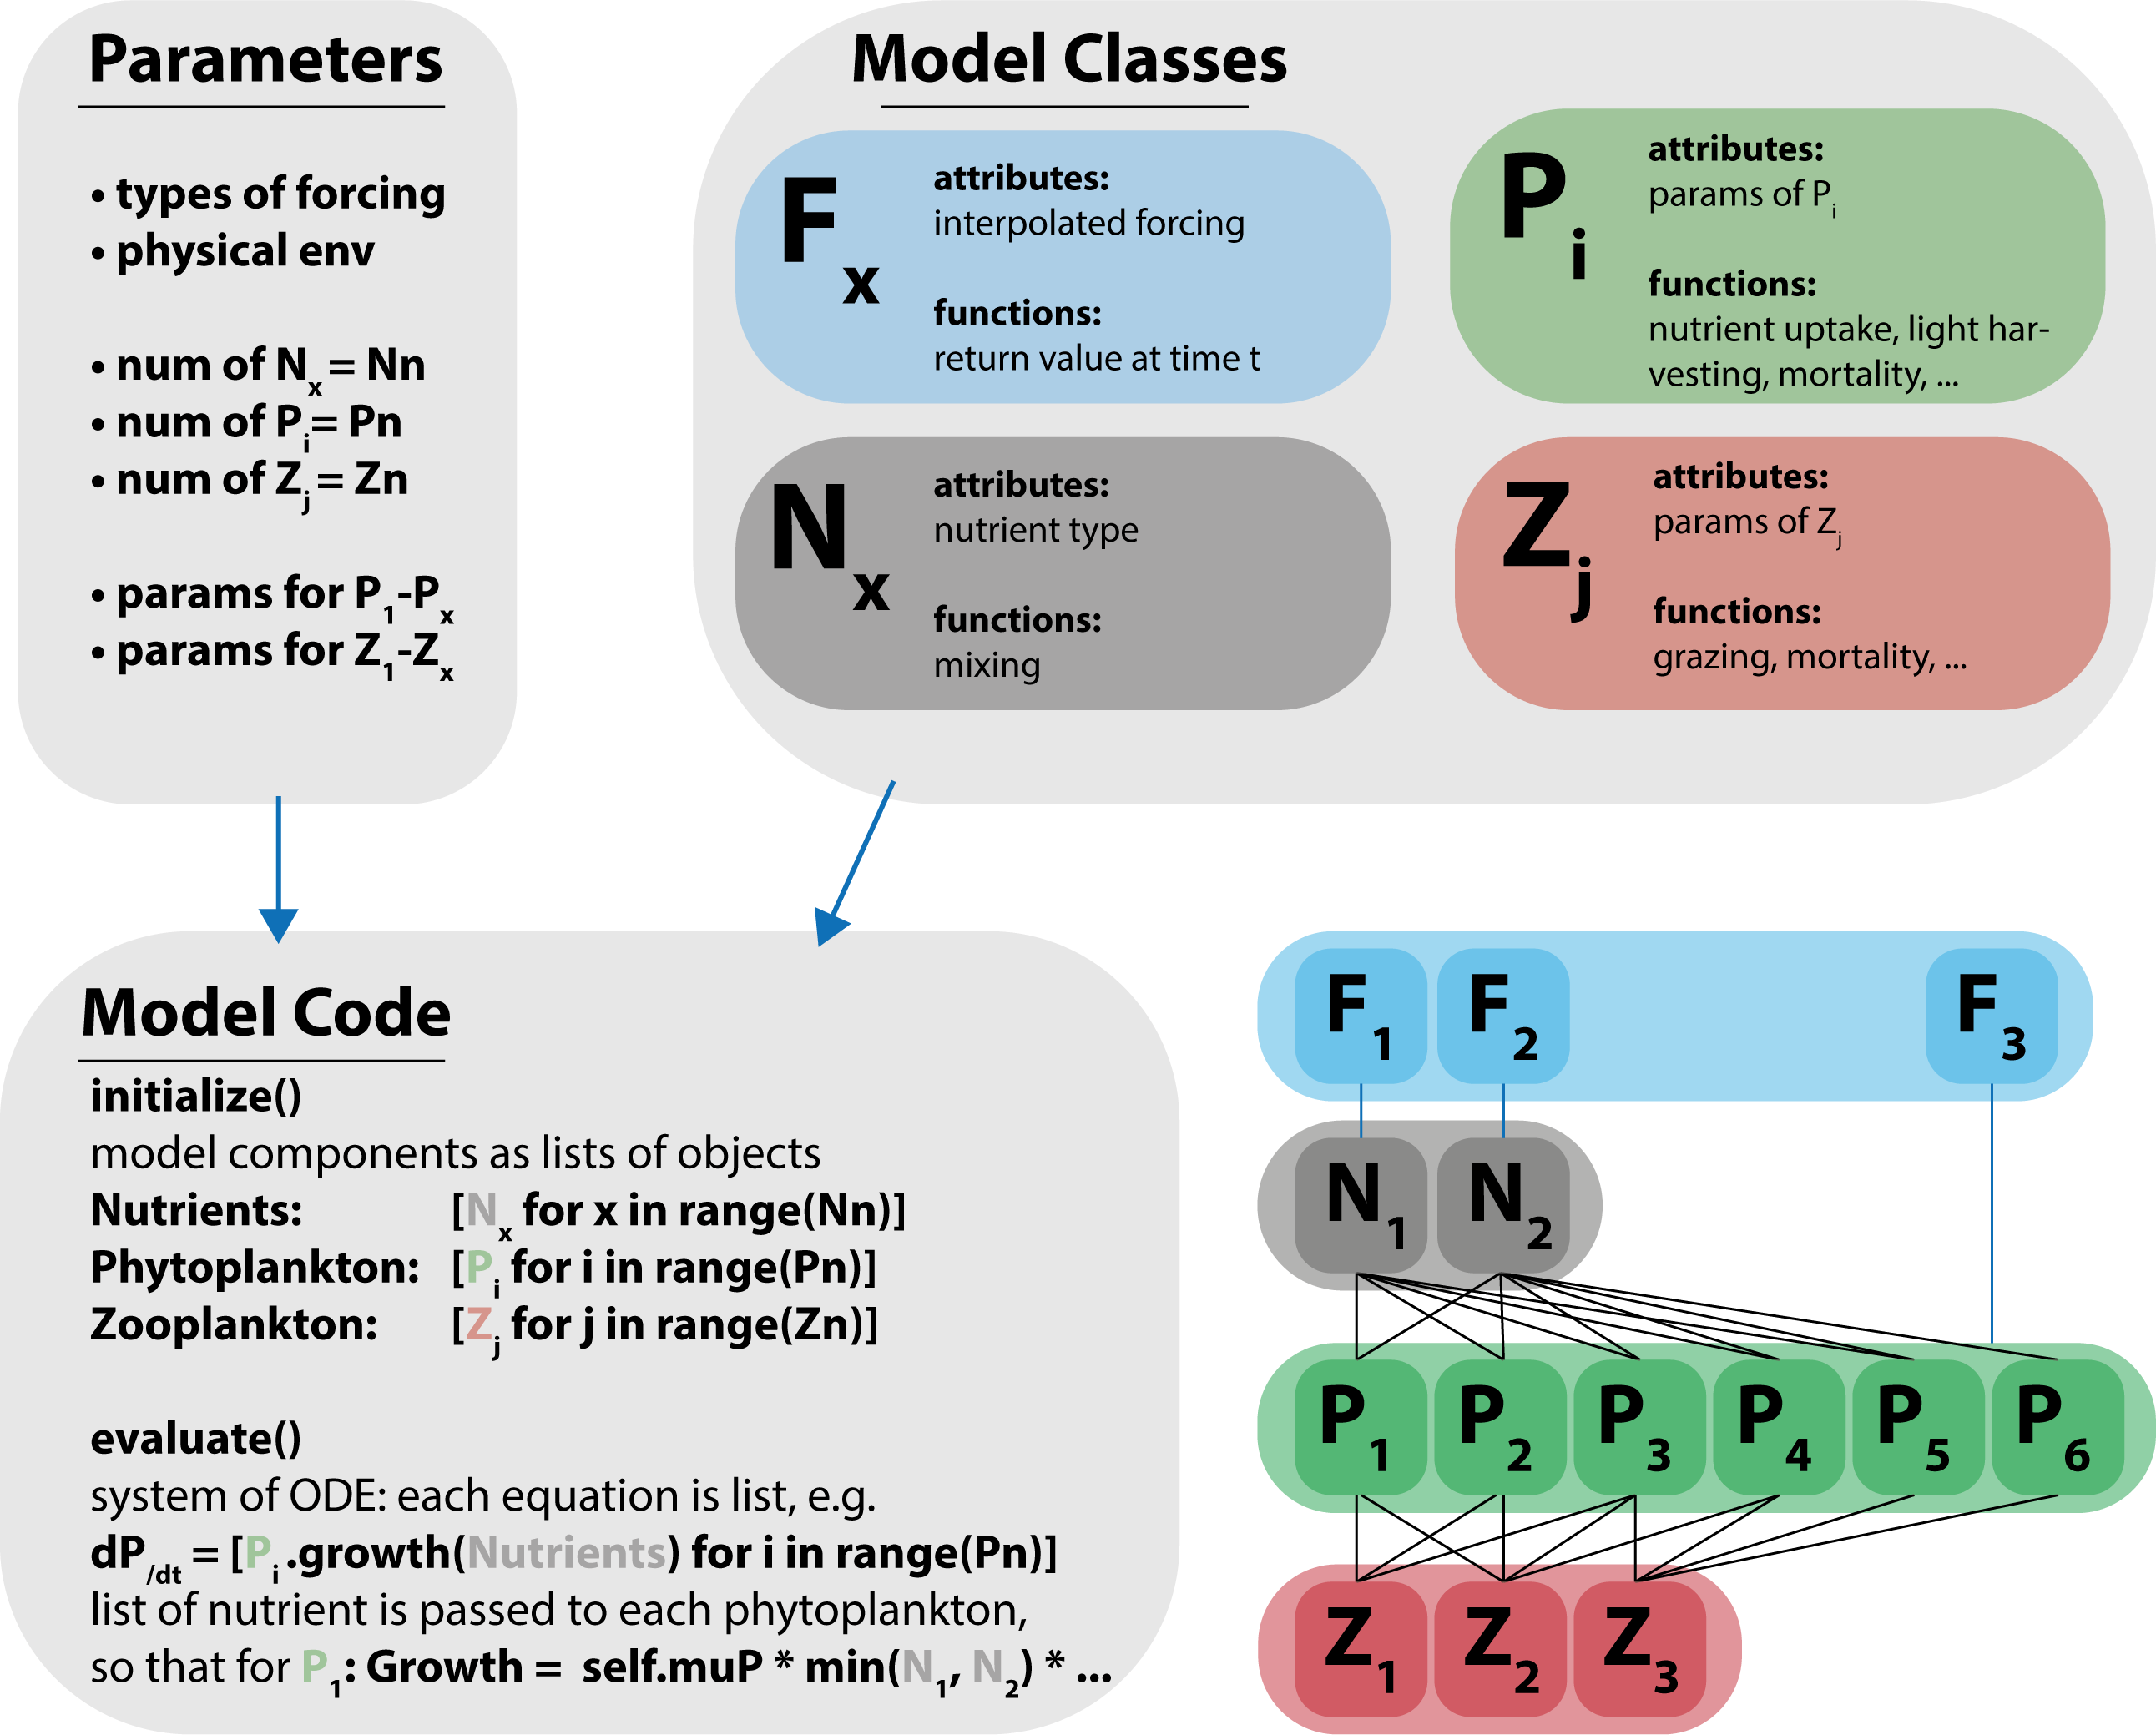
\includegraphics[trim = 0mm 0mm 0mm 0mm, clip, width=.9\linewidth]{./Chp22-Pre2/OOPmodelstructureDraft.png}
\caption[Scheme]{\small {Schematic of code structure for PhytoMFTM model. Square brackets ("[ ]") denote a list object in Python,"for i in range(x)" within brackets creates list of length x of whatever comes before. Model classes are used to store both the parameters associated with each instance, e.g. different nutrient uptake parameters for PFTs and the functions that are used within the ODE. Each equation is also a list structure that calls every instance of the required objects using list comprehensions, so that all interactions are calculated according to the number of model components that were initialized in the parameters.}}
\label{PrinComp}
\end{figure}


\noindent \small {\textbf{Model formulation and usage}}

xXXX

explain how to run the model!

XXXX

XXXX

XXX


End Methods here
